\chapter{Working Demonstration}
\label{ch:demo}

\section{Purpose and integrity}
The demonstration (\texttt{demo/app.py}, Streamlit) executes the \emph{actual}
exported checkpoint on real radar data in the datasets' native formats. It
contains no hard-coded, random or manually assigned predictions: every number on
the screen is computed by \texttt{inference.Bundle}, which uses the same
pre-processing code as training and evaluation.

\section{How to run}
\begin{lstlisting}[numbers=none]
pip install -r requirements.txt streamlit plotly
streamlit run demo/app.py          # opens http://localhost:8501
# command-line alternative
python src/inference.py --bundle checkpoints/stpt_lite_radhar \
                        --input demo/samples/radhar_test_jump.txt
\end{lstlisting}

\section{Application structure}
\begin{description}[nosep]
\item[Sidebar] select the trained model (RadHAR or MiliPoint bundle), a bundled
  test sample (ground truth known) or an uploaded file (\texttt{.txt} RadHAR ROS
  dump, \texttt{.npz} MiliPoint frames).
\item[1 Input \& pre-processing] frame/return/window counts; 3-D view of a raw window
  with antenna returns, gated clutter and kept person returns marked; the
  pre-processed model input coloured by time.
\item[2 Recognition] recording-level prediction (majority over 2-s windows),
  ground truth if known, single-window and whole-recording latency, per-window
  class probabilities and a probability-over-time heat map. A note explains that
  softmax probabilities are not calibrated accuracy.
\item[3 Noise robustness] choose a perturbation (jitter, dropout, sparsity,
  outliers, variable density, frame loss, combined), its level and seed; the app
  shows clean vs.\ noisy point clouds, both predictions, the percentage of
  unchanged window predictions and, when ground truth is known, the window
  accuracy before and after. The test-set robustness table is shown below.
\item[4 Model \& results] parameters, FP32/INT8 size, MFLOPs, latency, held-out
  test accuracy, macro-F1/precision/recall, confusion matrix, and the full
  architecture and training configuration.
\end{description}

\section{Input validation and error handling}
Unsupported extensions, text without RadHAR point records, npz files without
\texttt{pts}/\texttt{frame} or with wrong shapes, NaN/inf values, recordings
shorter than one 2-s window, and model/data mismatches (e.g.\ a RadHAR file with
the MiliPoint model) are rejected with a message instead of crashing the app.

\section{Bundled samples}
\texttt{demo/samples/} contains 12-s excerpts of five RadHAR \emph{official test}
recordings (one per class, in the original text format) and six 4-s MiliPoint
sequences from \emph{test subjects} 8 and 9. None of them was used for training
or model selection.

\section{Screenshots}
\begin{figure}[h]\centering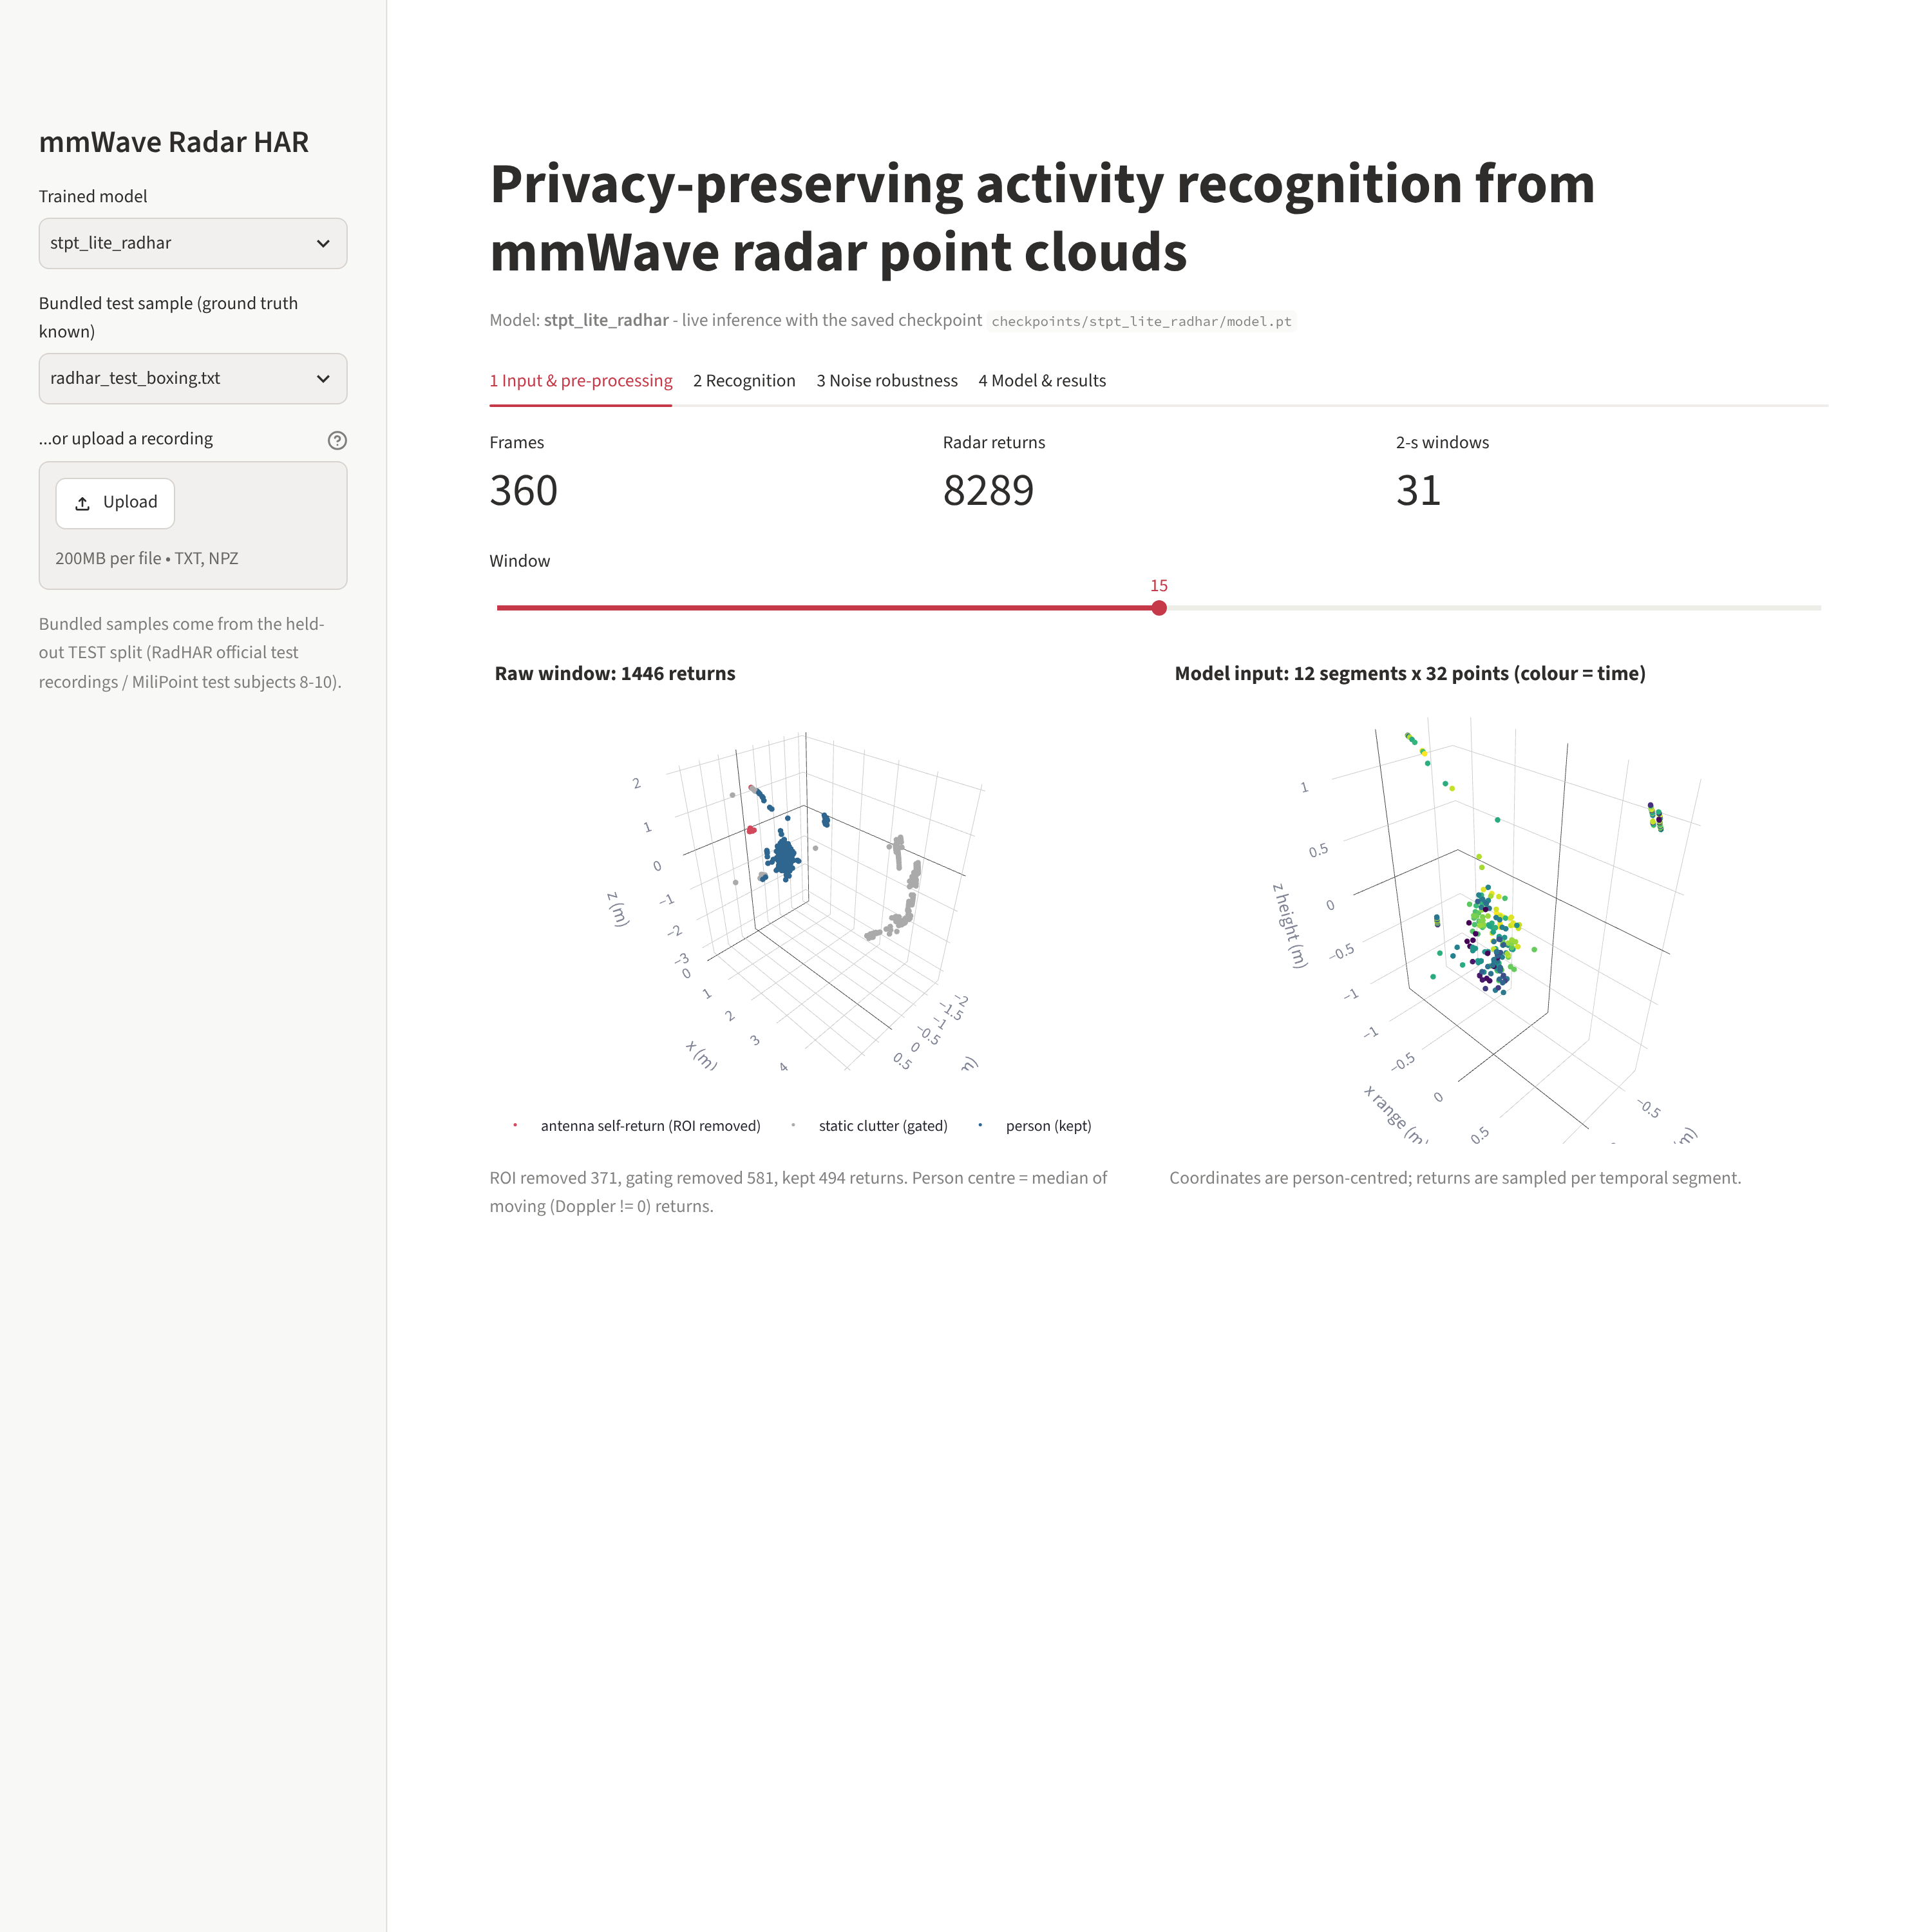
\includegraphics[width=0.92\textwidth]{demo/demo_input.png}\caption{Demonstration (real screenshot), Tab 1: raw window with antenna returns, gated clutter and kept person returns; pre-processed model input.}\label{fig:demo_input}\end{figure}
\begin{figure}[h]\centering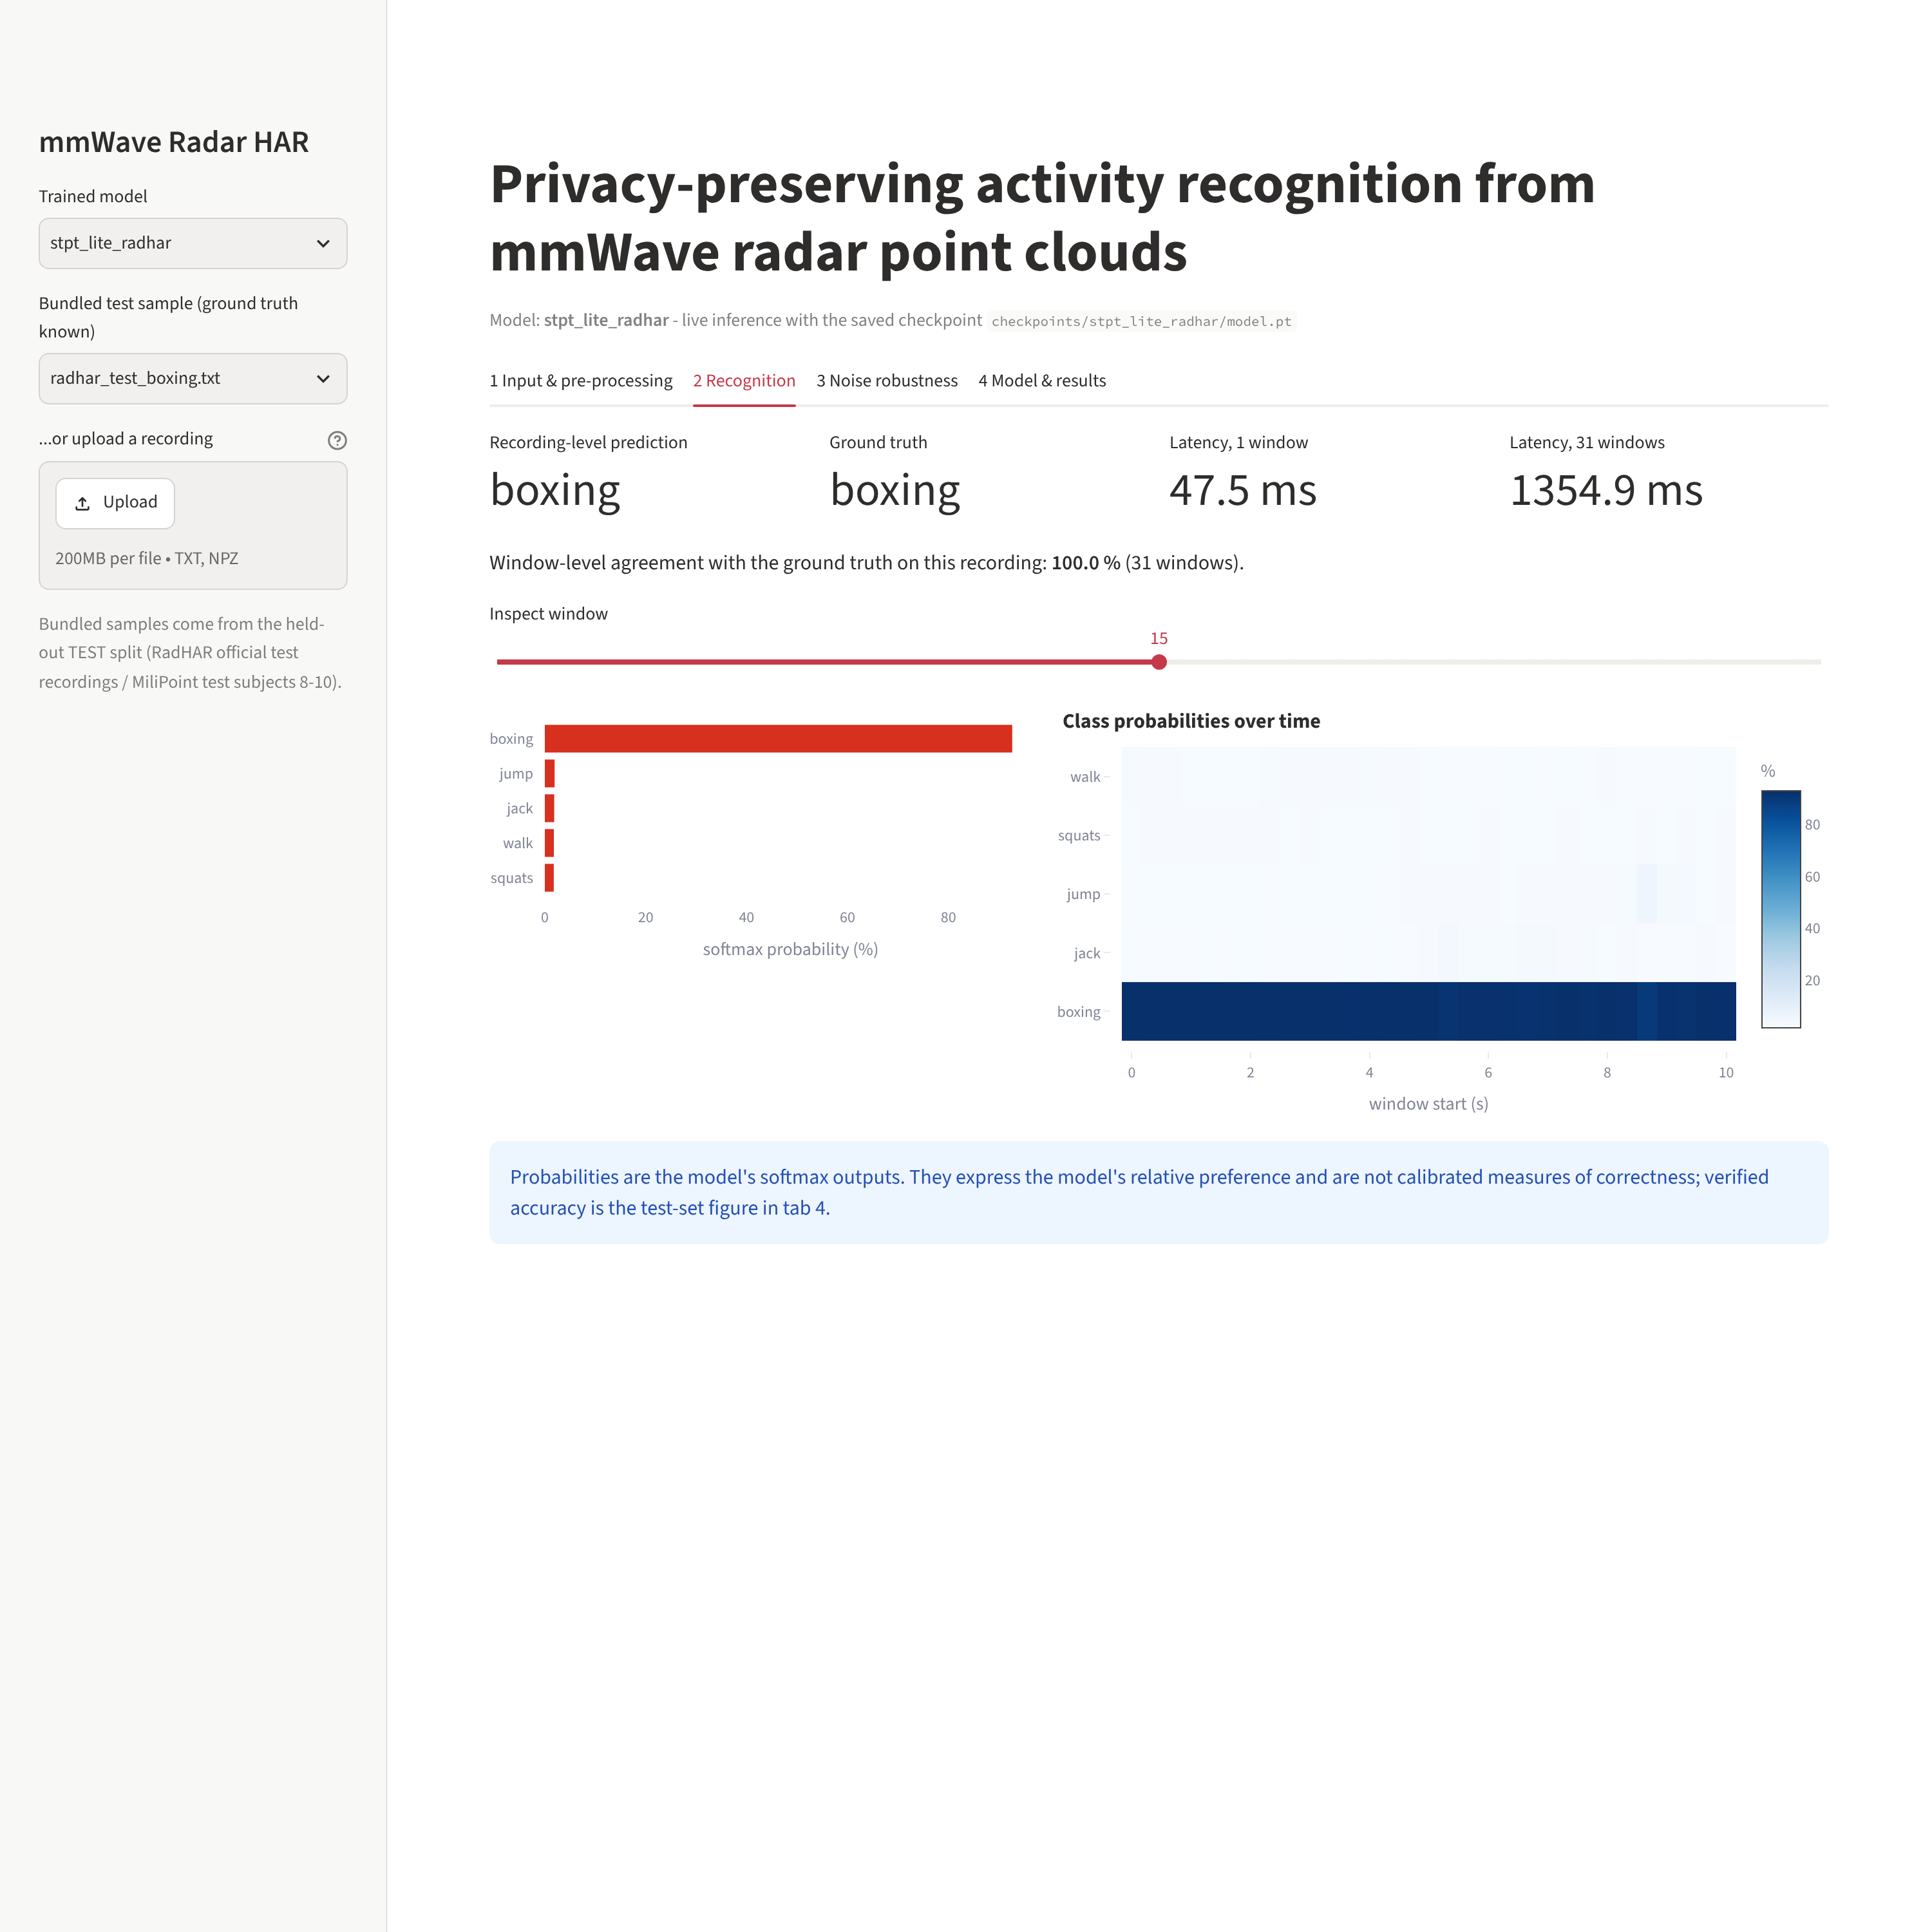
\includegraphics[width=0.92\textwidth]{demo/demo_recognition.png}\caption{Demonstration (real screenshot), Tab 2: live recording-level prediction, latency and per-window class probabilities.}\label{fig:demo_recognition}\end{figure}
\begin{figure}[h]\centering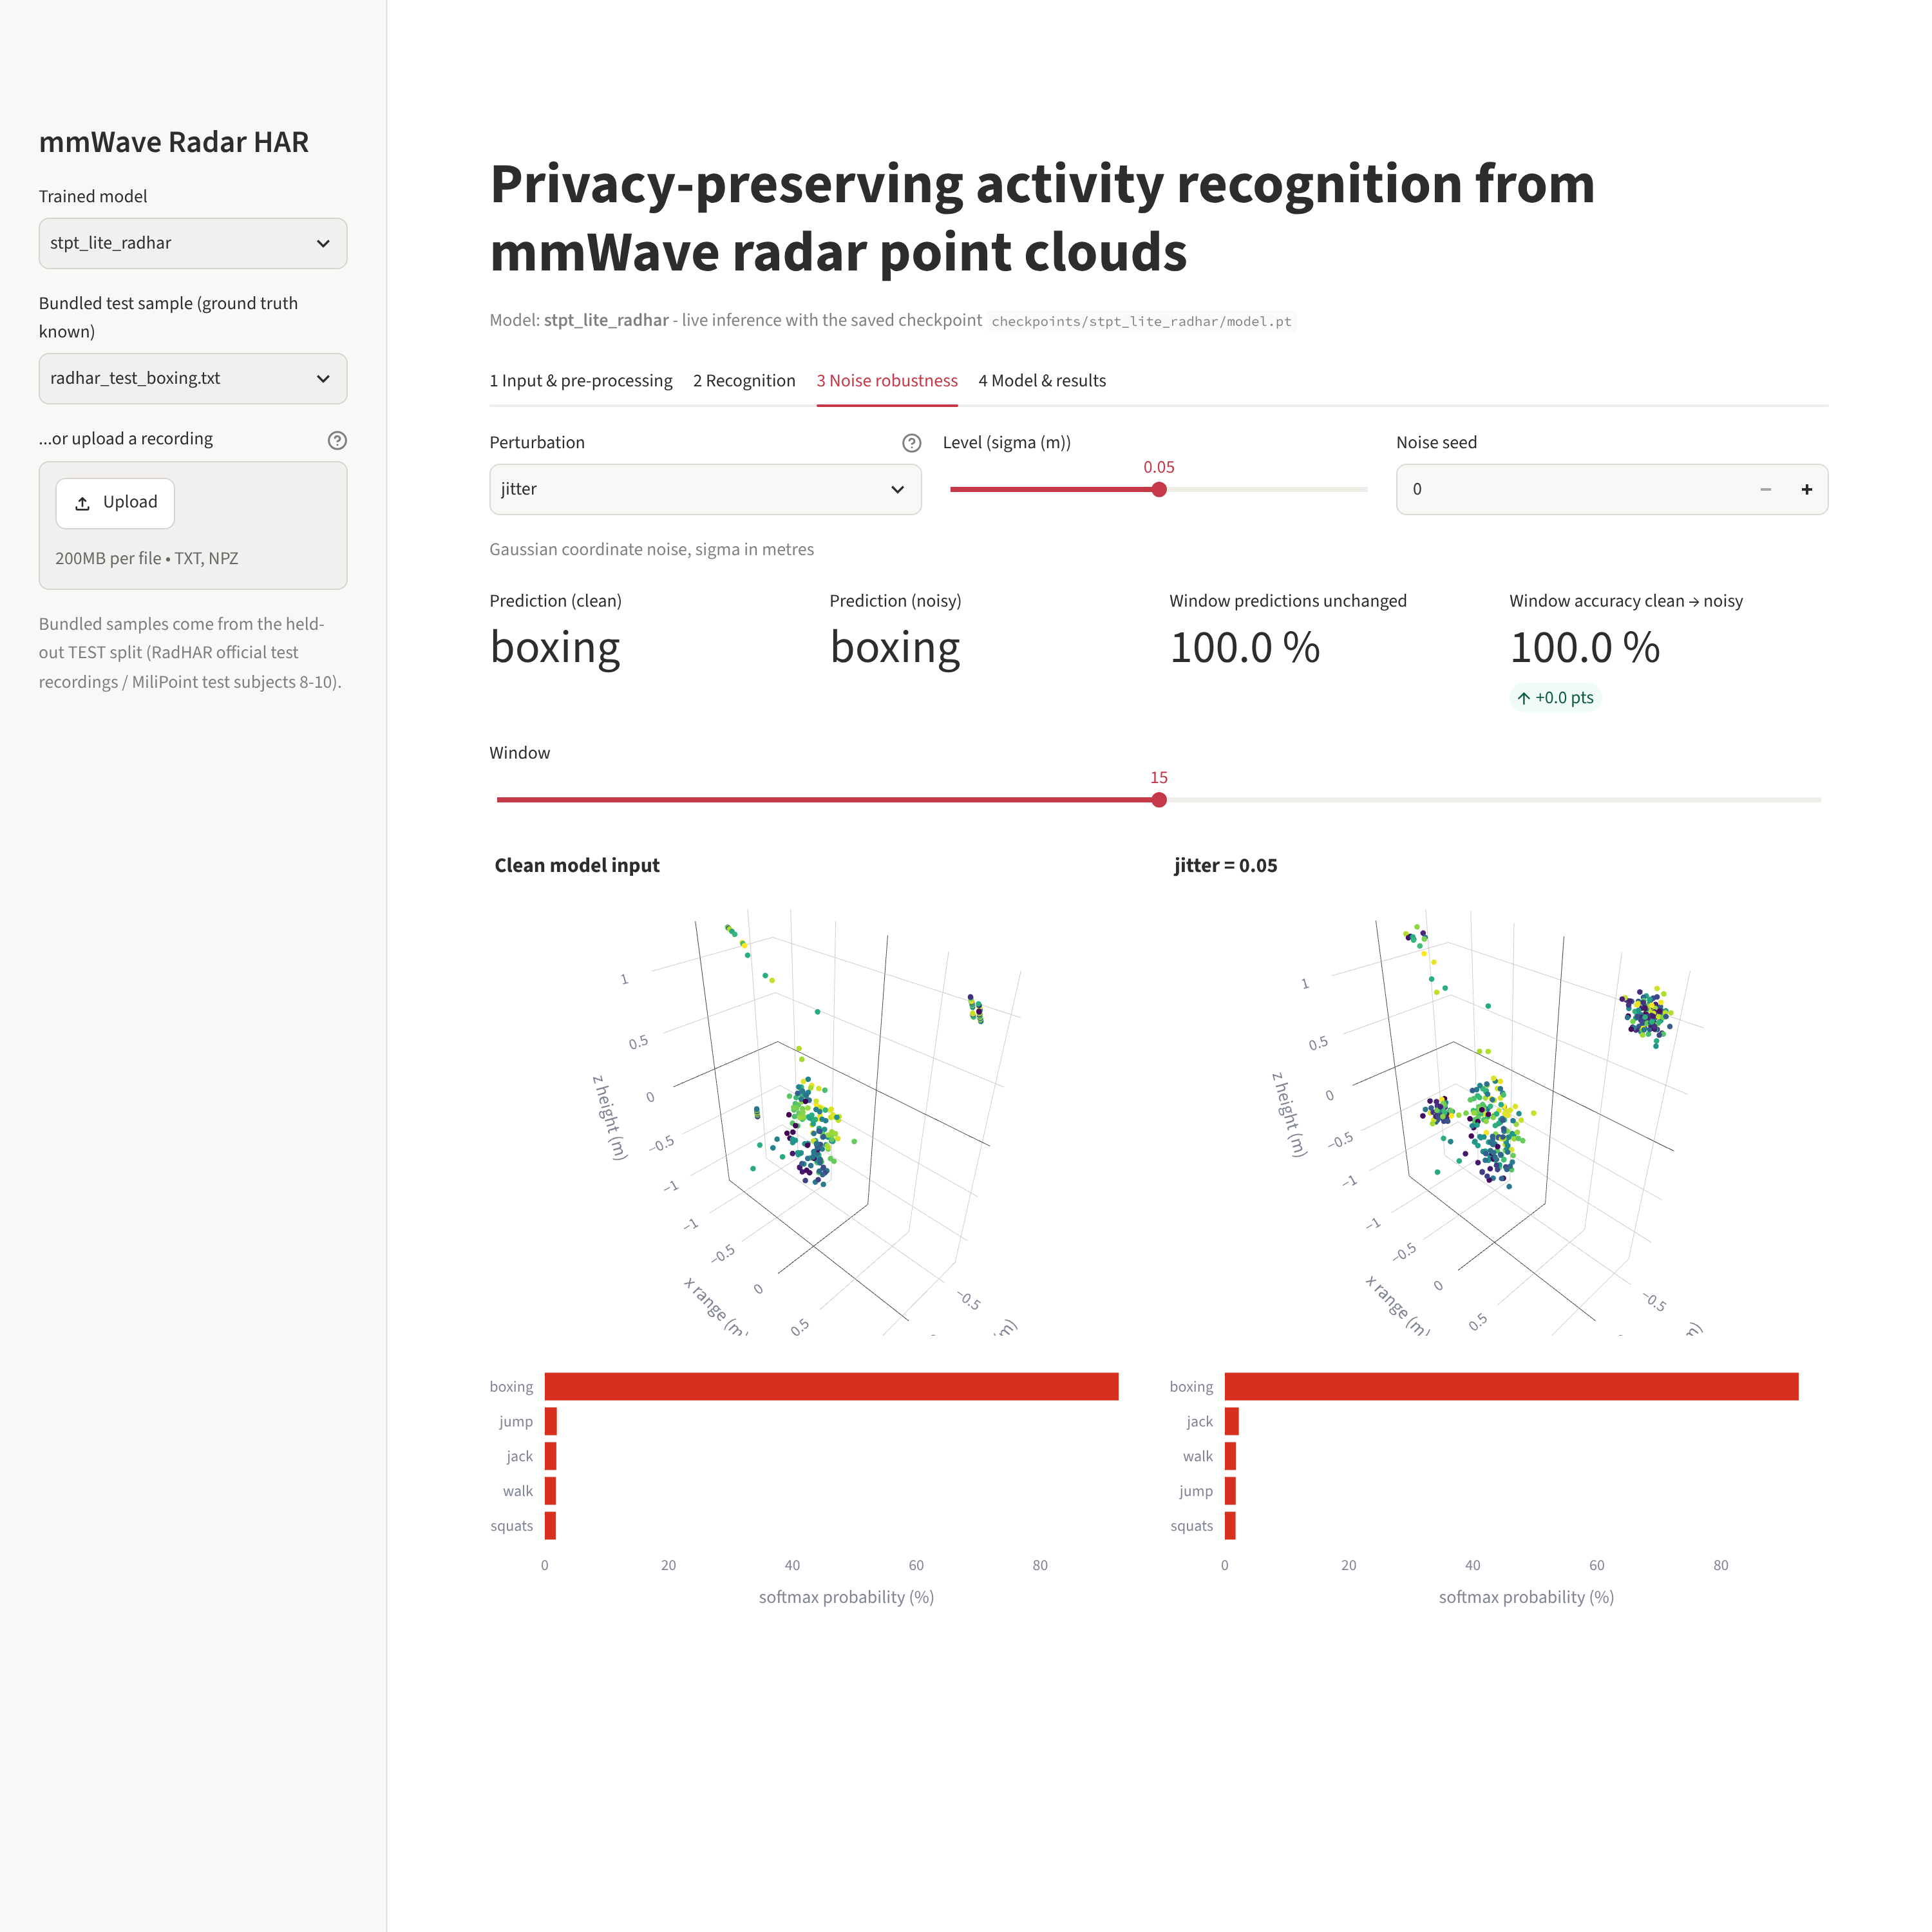
\includegraphics[width=0.92\textwidth]{demo/demo_noise.png}\caption{Demonstration (real screenshot), Tab 3: controlled noise injection; clean vs.\ noisy point cloud and predictions.}\label{fig:demo_noise}\end{figure}
\begin{figure}[h]\centering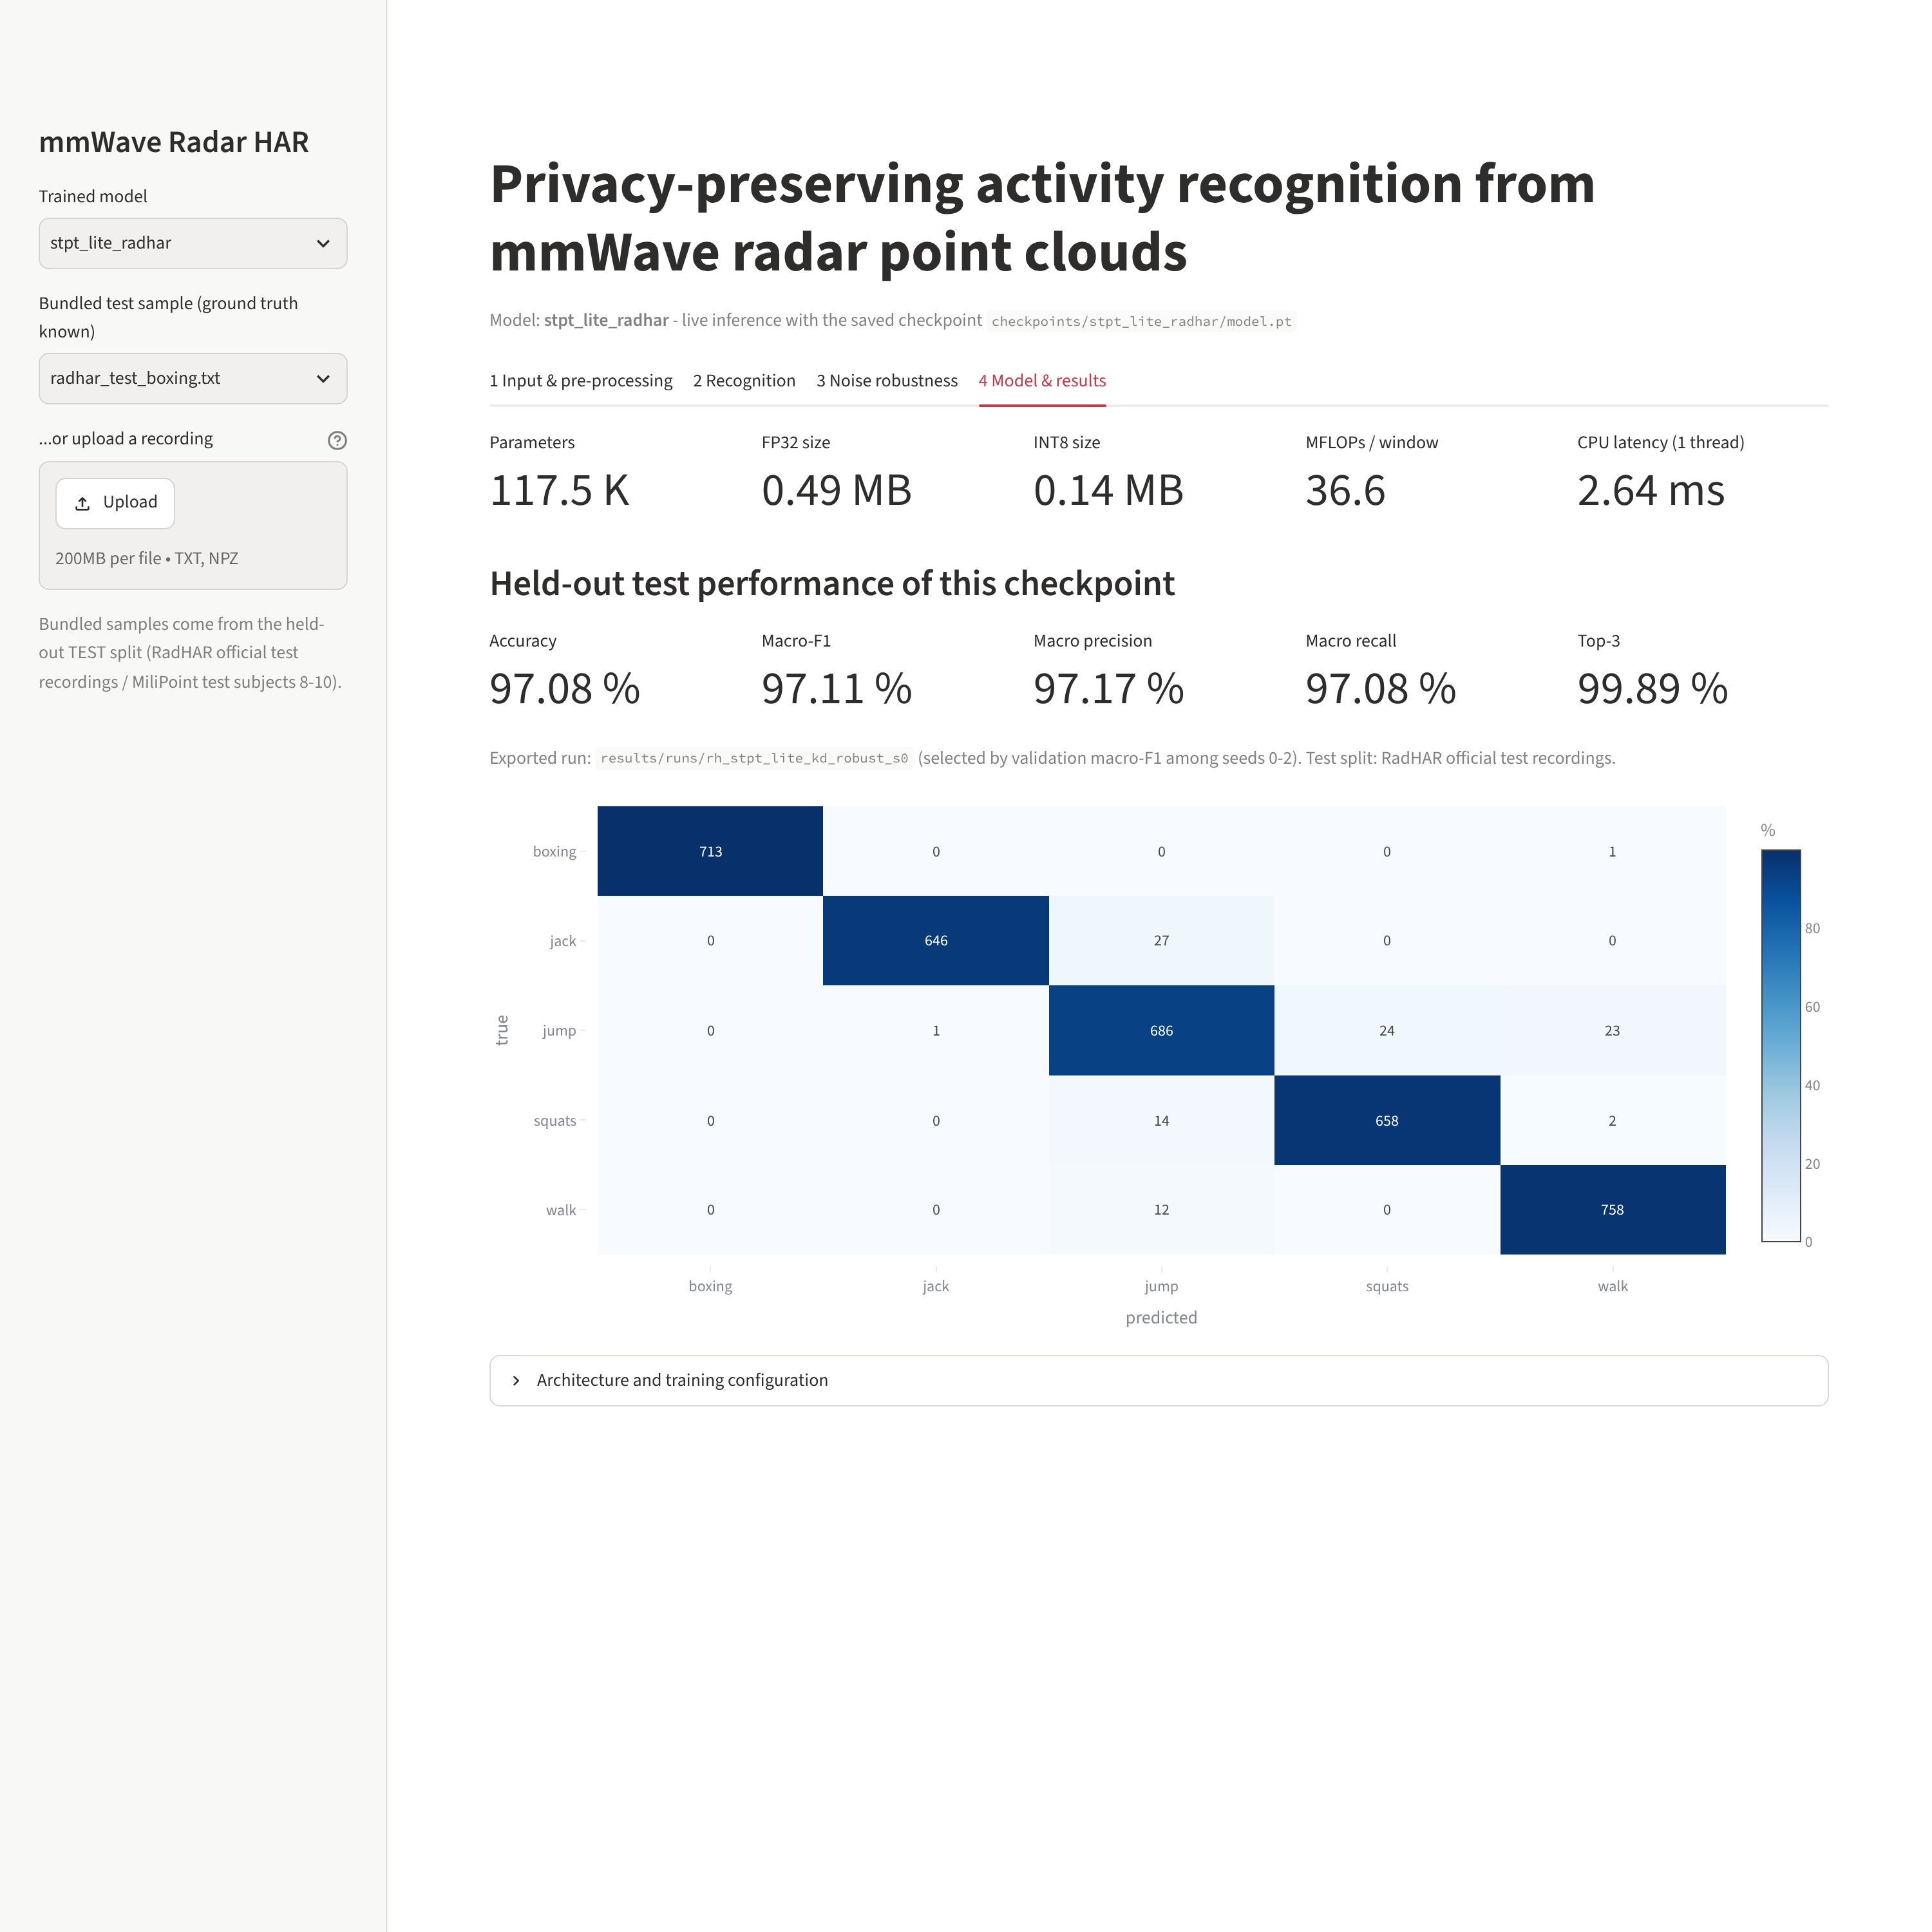
\includegraphics[width=0.92\textwidth]{demo/demo_model.png}\caption{Demonstration (real screenshot), Tab 4: model card with held-out test metrics and confusion matrix.}\label{fig:demo_model}\end{figure}
